% ******** Приклад оформлення документа за ДСТУ 3008-95 ********
% ******************** автор: Тавров Д. Ю. *********************

% зазначаємо стильовий файл, який будемо використовувати
\documentclass{udstu}

\addbibresource{refs.bib}

% починаємо верстку документа
\begin{document}

% створимо титульний аркуш
% за допомогою спеціальної команди
% \maketitlepage{params},
% де params --- це розділені комами пари "параметр={значення}"
\maketitlepage{
% StudentName --- прізвище, ініціали студента
	StudentName={Скорденко Д. О.},
% StudentMale --- стать студента (true, якщо чоловік, false --- якщо жінка)
	StudentMale=true,
% StudentGroup --- група студента
	StudentGroup={КМ-01},
% Title --- назва
	Title={Пояснювальна записка до курсового проекту\\ із дисципліни \\ \invcommas{Алгоритми і системи комп'ютерної математики}\\
	на тему \\ \invcommas{Автоматична аннотація зображень за допомогою нейронних мереж}},
% SupervisorDegree --- науковий ступінь, учене звання керівника роботи
% якщо наукового ступеня немає, можна відповідний рядочок пропустити
	SupervisorDegree={асистент кафедри ПМА},
% SupervisorName --- прізвище, ініціали керівника роботи
	SupervisorName={Ковальчик-Химюк Л. О.}
}


% Створюємо анотацію
\abstractUkr

В даній роботі описано мультимодальну систему маркування зображень, в якій зроблено акцент на трьох апспектах:
висока точність, використання тексту в якості додаткової інформації, явна підсистема для передбачення к-сті лейблів.
Всі ці рішення значно підвищують точність в порівннянні із існуючими рішеннями.


\shortings

\begin{itemize}[*]
	\item DNN - Глибинна нейронна мережа (Deep Neural Network)
	\item CNN - Згорткова нейронна мережа (Convolutional Neural Network)
	\item RNN - Рекурсивна нейронна мережа (Recursive Neural Network)
	\item Анотація зображень, маркування зображень, мульти-лейбел класифікація - взаємозамінні поняття
\end{itemize}


% створюємо зміст
\tableofcontents


% створюємо перший розділ роботи
\chapter{Вступ}

Задача класифікації - це одна із основних задач в аналізі зображень, вона полягає
у присвоєнні кожному зображенню один із класів. Таким чином дане формулювання накладає
обмеження - зображення містить тільки один об'єкт. Поява DNN \cite{dnn-cls}
та її подальший розвитком у CNN \cite{cnn-cls-1,cnn-cls-2} разом із створенням
великих датасетів як-от ImageNet \cite{deng2009imagenet} дало змогу вирішувати задачу
класифікації зображень значно швидше і якісніше ніж люди.

Зрозуміло, що зображення - це той тип даних, який у абсолютній більшості випадків містить більше одного об'єкта.
Для поглиблення опису існує задача маркування зображень (image labeling). На відміну від
класифікації, вона полягає у маркуванні зображення більше ніж одним класом. Таким чином
якість опису зображення кратно зростає у порівннянні із звичайною класифікацією,
однак привносить декілька складних завдань.

По-перше, наявність декількох класів у одного зображення створює можливість
описувати значно ширший спектр візуальної інформації: різні об'єкти, стилі, дії, і тд.
Поява великих хостингів зображень таких як Imgur, Flickr, та ін., де користувачі можуть
як завантажувати різноманітні зображення, так і додавати до них описову інформацію у вигляді
тегів / анотацій, дала змогу створити досить різноманітні датасети: ImageNet \cite{deng2009imagenet},
MS-COCO \cite{cocodataset}, NUS-WIDE \cite{nus-wide-civr09}, та ін.

По-друге, анотація зображень передбачає не лише маркування більше ніж одним класом,
а і передбачення к-сті класів. Для опису зображенням із широким спектром понятть необхідно $N$ класів,
для зображення із простим вмістом - 2-3 класи.

По-третє, анотація зображень потребує оцінки якості проведеного маркування. Оскільки будь який
датасет буде містити в собі дизбаланс класів в тій чи іншій мірі, важливо оцінювати маркування із
урахуванням цього.

Все це робить задачу маркування зображення досить складною.


\chapter{Огляд існуючих рішень}

\paragraph{\textbf{Базове рішення}\\}

Базовим рішенням для більшості робіт із маркування зображення є використання CNN.
Більшість робіт використовує різні архітектури ResNet \cite{resnet}, AlexNet \cite{alexnet}, GoogleNet \cite{googlenet}.
Спільним між ним є те що вони вже натреновані на великому датасеті, здебільшого ImageNet \cite{deng2009imagenet}.
Для адаптації моделі до обраного контексту така модель дотреновуєтсья (fine tune), замінюючи базовий класифікатор на
такий же простий із адаптованою к-стю вихідних класів \cite{cnn-labeling-1}, або ж на більш складний класифікатор (який надає більш точні результати) \cite{cnn-labeling-2}. Це працює завдяки тому, що всі архітектури сучасних CNN моделей є багатошаровими,
і в них перші шари розпізнають базові особливості (features) зображення, які можна навіть візуалізувати, однак
останні шари вивчають більш глибинні особливості зображення, таким чином роблячи модель більш універсальною при зміні
класифікатора.

\paragraph{\textbf{Додаткова інформація}\\}

Більш нові роботи також розглядають додавання сторонньої інформації для класифікації зображень.
Існує два основних підходів:

\begin{enumerate}
	\item Семантичний аналіз лейблів.
	Даний підхід аналізує зв'язок між різними класами.
	Схожі за контекстом лейбли знаходяться поруч (наприклад: риба, вода)
	\cite{cnn-semantic-1, cnn-semantic-2}
	\item Аналіз додаткової інформації.
	Даний підхід аналізує додаткову до зображення інформацію.
	Це може бути як текстова інформація (теги / анотації) \cite{cnn-side-2},
	так і метадані зображення \cite{cnn-side-1,cnn-side-3}
\end{enumerate}

\paragraph{\textbf{К-сть лейблів}\\}

Всі наведені вище роботи розглядаєють задачу вибору к-сті лейблів як найкращі $k$ (top $k$) маркувань.
$k$ найбільше ймовірних класів, де $k$ - наперед задана константа. Очевидно, що такий вибір к-сті класів не є
оптимальним, так як більш змістовні зображення будуть містити менше описової інформації і навпапки - менш змістовні будуть
містити лишню інформацію, яка до того ж може не мати нічого спільного із цим зображенням (\figurename{\ref{figure:test-topk}})

\begin{figure}[!ht]
	\centering
	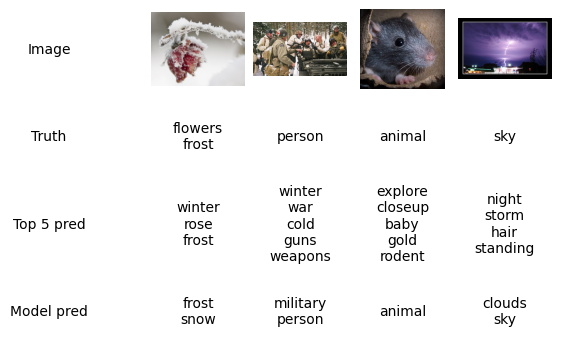
\includegraphics[width=0.9\textwidth]{PNG/test-topk}
	\caption{Приклад адаптивної к-сті лейблів}
	\label{figure:test-topk}
\end{figure}

Один із сучасних підходів як-от CNN-RNN \cite{cnn-rnn},
розглядає задачу маркування як задачу перекладу зображення в текст (image to text),
де CNN - це кодувальник (encoder), а RNN (decoder) автоматично виконує як задачу маркування,
так і задачу динамічного вибору кількості лейблів, однак є певні обмеження
накладенні на порядок класів.


\chapter{Моделювання}

На основі проведного аналізу альтернатив, дана робота пропонує розглянути
мультимодальну систему, яка складається із чотирьох компонентів (\figurename{\ref{figure:composite}})

\begin{figure}[!ht]
	\centering
	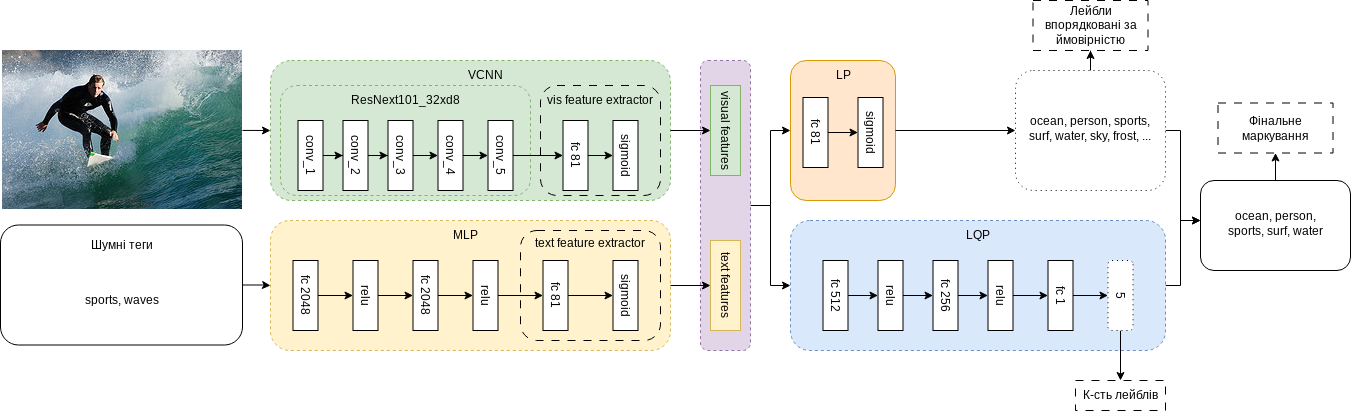
\includegraphics[width=0.9\textwidth]{PNG/composite}
	\caption{Архітектура композитної системи}
	\label{figure:composite}
\end{figure}

\section{VCNN}

Модель (\figurename{\ref{figure:composite}}) призначена для вивчення особливостей (features) із зображення.
Отримує на вхід піселі зображення $I$, у формі матриці розмірності $(B,C,W,H)$, де
$B$ - к-сть зображень у групі для тегування,
$C$ - к-сть каналів у зображеннях зазвичай 1 або 3, Grey або RGB відповідно,
$W,H$ - розмірність зображень.

За базове рішення використовуєтсья ResNext101\_32x8d \cite{resnext} (сучасна версія resnet),
із адаптованим класифікатором.

На виході даної моделі ми отримуємо вектор вірогідностей $vf$ (visual feature vector),
який вказує вірогідність маркування зображення класом $j$.


\section{MLP}

MLP (\figurename{\ref{figure:composite}}) - аналізує текстові особливості (text features) тегів до зображення.
Теги до зображення $i$ репрезентуються як бінарний вектор $I = [1,0,1,0, ..., N]$,
де 1 - це наявність тегу, а $N$ - к-сть тегів.

На виході даної моделі ми отримуємо вектор $tf$ вірогідностей (text feature vector),
який вказує вірогідність маркування зображення класом $j$.


\section{LP}

LP (\figurename{\ref{figure:composite}}) - аналізує вектор вірогідності $v$, який є композицією векторів $vf$ та $tf$.

На виході даної моделі ми отримуємо вектор вірогідностей


\section{LQP}

Модель LQP аналізує кількість лейблів на основі вектору вірогідностей $v$, який є композицією векторів $vf$ та $tf$.

Існує два підходи до визначення к-сті за допомогою нейронних мереж: класифікація та регресія.
LQP - регресійна модель.

На виході даної моделі є число, яке вказує на ксть лейблів у зображенні.

% створюємо Висновки
\conclusions

\printbibliography

\end{document}
